\documentclass[11pt]{article}
\usepackage[review]{acl}

\usepackage{times}
\usepackage{latexsym}
\usepackage[T1]{fontenc}
\usepackage[utf8]{inputenc}
\usepackage{microtype}
\usepackage{graphicx}
\usepackage{amsmath,amssymb,amsthm}
\usepackage{bm}
\usepackage{booktabs}
\usepackage{array}
\usepackage{makecell}
\renewcommand{\cellset}{\renewcommand{\arraystretch}{0.85}}
\usepackage{multirow}
\usepackage[table]{xcolor}
\usepackage{enumitem}
\usepackage{float}
\usepackage{algorithm}
\usepackage{algpseudocode}
\usepackage{xspace}
\usepackage{pifont}

\definecolor{rowours}{HTML}{EAF2FC}
\definecolor{refgray}{HTML}{7A7973}
\definecolor{dltc}{HTML}{8A3B12}
\newcommand{\dlt}[1]{{\scriptsize\textcolor{dltc}{(#1)}}}
\newcommand{\std}[1]{{\scriptsize$\pm$#1}}
\makeatletter\newcommand{\inputtable}[1]{\@@input #1 }\makeatother

\newtheorem{theorem}{Theorem}
\newtheorem{proposition}{Proposition}
\newtheorem{lemma}{Lemma}
\theoremstyle{remark}
\newtheorem*{remark}{Remark}

\newcommand{\method}{GivenRL\xspace}
\newcommand{\cA}{\mathcal{A}}
\newcommand{\Aplus}{\mathcal{A}^{+}}
\newcommand{\ind}{\mathbf{1}}
\newcommand{\shat}{\hat{s}}
\newcommand{\astar}{a^{\star}}
\newcommand{\aminus}{a^{-}}
\newcommand{\atilde}{\tilde{a}}
\newcommand{\ahat}{\hat{a}}
\newcommand{\E}{\mathbb{E}}
\newcommand{\Kmax}{K_{\max}}

\title{Every Question Carries Its Own Answer Key:\\Label-Free Reinforcement Learning from Verifiable Givens}

\author{Anonymous ACL submission}

\begin{document}
\maketitle

\begin{abstract}
Label-free reinforcement learning trains reasoning models on problems without reference answers. Current methods reward agreement: with the model's majority vote, across paraphrases of the question, with a peer model, or with a verifier trained on votes. In a two-outcome model of GRPO training, we show that every reward of this kind keeps the all-wrong state stable, so a model that is confidently wrong on a problem is trained to stay wrong. We draw the signal from text the model did not write, namely the quantities the problem gives. For a candidate answer, we hide one given, state the candidate as a fact, and ask the same policy to recover the hidden value, which is an exact label. Recovery succeeds more often when the stated answer is correct. \method rewards forward answers by their recovery rate and trains inverse solving on answers that pass a consistency check against a known-wrong control. In the two-outcome model, the correct answer becomes the only stable state of training whenever the recovery gap is positive. On Qwen3.5-4B/9B-Base and Olmo-3-7B trained on unlabeled DAPO-Math-17k, \method exceeds the strongest label-free baseline by 1.4 to 2.0 points on an eight-benchmark math average and comes within 1.0 point of ground-truth GRPO.It fixes 36\% of the problems on which the base model is confidently wrong, against 9\% for TTRL.
\end{abstract}

%=====================================================================
\section{Introduction}
%=====================================================================

Reinforcement learning with verifiable rewards (RLVR) is the standard way to improve the reasoning of language models \citep{shao2024deepseekmath,guo2025deepseekr1}, and it needs a reference answer for every training problem. Reference answers are expensive for hard problems and absent for unsolved ones, so a growing line of work trains on unlabeled problems instead \citep{zuo2025ttrl,prabhudesai2025rent,zhao2026intuitor}.

These methods all take their correctness signal from the beliefs of the models being trained. TTRL rewards agreement with the policy's majority vote \citep{zuo2025ttrl}. Co-rewarding and Self-Harmony reward agreement across paraphrases \citep{zhang2026corewarding,wang2026selfharmony}, Co-RL rewards agreement with an independently trained peer \citep{yang2026corl}, and CoVerRL trains a verifier on majority votes \citep{pan2026coverrl}. Each step reduces correlated errors; none adds information the models lack. When the majority answer is wrong, the reward pushes the policy toward it. This is the reinforcement-learning form of confirmation bias in self-training \citep{arazo2020pseudo}, which \citet{pan2026coverrl} call the consensus trap. We show that the trap is structural. In a two-outcome model of GRPO, any reward whose ranking of answers is decided by the votes of models that are all wrong keeps the all-wrong state stable (Section~\ref{sec:trap}). Better views move the boundary of the wrong basin and leave the basin in place (Figure~\ref{fig:teaser}b). Qwen3.5-4B-Base is confidently wrong on 14\% of DAPO-Math-17k problems, and TTRL fixes 9\% of them.

\begin{figure}[t]
  \centering
  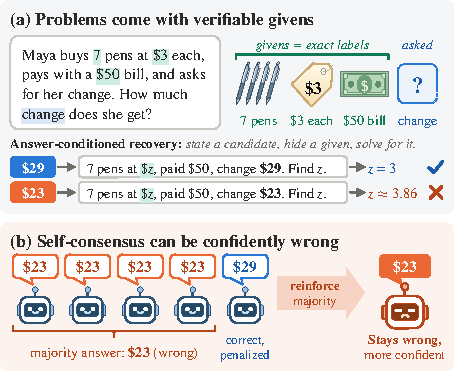
\includegraphics[width=\columnwidth]{figures/fig1_teaser.pdf}
  \caption{\textbf{(a)}~An inverse problem hides one given, states a candidate answer as a fact, and asks for the hidden value. The correct change (\$29) gives back the price \$3; the wrong change (\$23) gives $27/7\approx3.86$. \textbf{(b)}~Expected update of the probability $p$ of the correct answer in the two-outcome model ($G{=}8$). Rewarding the policy's own majority vote drives every problem with $p<1/2$ to $p=0$ (shaded). A peer that is correct more often ($p+0.15$) moves the boundary to $p=0.36$ and leaves $p=0$ stable. \method's update is the ground-truth update scaled by $\psi=0.87$, evaluated at the pilot recovery rates.}
  \label{fig:teaser}
\end{figure}

A math problem, however, states several facts and leaves one quantity unknown, and a correct answer lets us recover those facts. In Figure~\ref{fig:teaser}a, Maya buys 7 pens at \$3 each, pays with a \$50 bill, and asks for her change. Write a candidate change into the problem, hide the price, and ask for it: a change of \$29 gives back \$3, and a wrong change of \$23 gives about \$3.86. The hidden price is an exact label because we removed it ourselves. \citet{weng2023selfverification} and \citet{jiang2024fobar} used this forward-backward check to rerank answers at inference time; we use it to produce training signal. On 512 unlabeled DAPO-Math problems, Qwen3.5-4B-Base recovers a masked given 58\% of the time under the correct answer and 21\% under its most frequent wrong answer. On the problems where its majority vote is wrong, the rates are 54\% and 23\%, so the signal survives on the problems where agreement-based rewards point the wrong way.

\method turns this gap into a reward (Figure~\ref{fig:method}). The policy answers a problem; for each candidate and a few givens, a template builds an inverse problem; the same policy solves it, and the recovery rates score the forward answers. The inverse rollouts carry exact rewards, so they also train the policy, but only for the leading candidate and only after it beats a perturbed, known-wrong answer by a margin. This consistency gate keeps the inverse solver reading the answer it is given. In the two-outcome model, \method's expected update is the ground-truth update scaled by a positive factor whenever recovery favors the correct answer. We call the general setting reinforcement learning with verifiable givens (RLVG). Our contributions are:
\begin{itemize}[leftmargin=*,itemsep=1pt,topsep=2pt]
  \item \textbf{A diagnosis.} Rewards decided by model votes, including cross-view, cross-model and vote-trained verifier rewards, keep the all-wrong state stable (Proposition~\ref{prop:trap}).
  \item \textbf{A reward source.} RLVG labels answer-conditioned inverse problems with the problem's givens. \method's anchor-scored reward and gated inverse training make the correct answer the unique stable state when the anchor gap is positive (Theorem~\ref{thm:stable}).
  \item \textbf{Evidence.} On three backbones, eight math and five out-of-domain benchmarks, \method is the strongest label-free method and gains most on confidently wrong problems: it fixes 50\% of those whose givens respond to the answer, against 51\% for ground-truth GRPO.
\end{itemize}

%=====================================================================
\section{Related Work}
%=====================================================================

\paragraph{Label-free RL for reasoning.}
Confidence rewards use low token entropy \citep{prabhudesai2025rent,agarwal2025entropy}, low semantic entropy \citep{zhang2025empo} or high self-certainty \citep{zhao2026intuitor}. Vote rewards use the majority over sampled answers \citep{zuo2025ttrl,shafayat2025selftrain}, the training-time form of self-consistency \citep{wang2023selfconsistency}. Later work keeps the vote and adds a novelty bonus \citep{zhou2025evolrl}, down-weights low-consensus pseudo-labels \citep{yu2026restrain}, or masks answer tokens out of the update \citep{ye2026omgrpo}. Cross-view and cross-model methods pool votes across paraphrases \citep{zhang2026corewarding,wang2026selfharmony} or across independently trained models \citep{yang2026corl}. Table~\ref{tab:taxonomy} groups these methods by the source of their correctness signal.

\begin{table}[t]
  \centering
  \small
  \setlength{\tabcolsep}{4pt}
  \begin{tabular}{@{}>{\raggedright\arraybackslash}p{2.05cm}>{\raggedright\arraybackslash}p{2.95cm}>{\raggedright\arraybackslash}p{1.85cm}@{}}
    \toprule
    Signal source & Methods & All-wrong state stable? \\
    \midrule
    Own confidence & RENT, Intuitor, EMPO & yes \\
    Own votes & TTRL, EVOL-RL, RESTRAIN, OM-GRPO & yes \\
    Votes across views & Co-rewarding, Self-Harmony & yes, smaller basin \\
    Votes across models & Co-RL & yes, smaller basin \\
    Verifier fit to votes & CoVerRL & yes, when its labels err \\
    \midrule
    Formal checker & JURY-RL & no, where formalized \\
    \rowcolor{rowours}Problem givens & \method (ours) & no, if $\Delta>0$ \\
    \bottomrule
  \end{tabular}
  \caption{Label-free rewards grouped by where their correctness signal comes from. The last column summarizes Section~\ref{sec:method}.}
  \label{tab:taxonomy}
\end{table}

\paragraph{Verification during training.}
Models rarely correct their own reasoning without external feedback \citep{huang2024cannot}. CoVerRL trains a verifier on majority-vote labels \citep{pan2026coverrl}, which are wrong exactly where the vote is wrong. JURY-RL gates rewards with a Lean prover \citep{chen2026juryrl}; its signal is sound where autoformalization succeeds and requires a 32B-scale formalizer and prover. \method's second role learns from labels taken from the problem text.

\paragraph{Backward reasoning and round trips.}
Self-verification masks a condition and checks whether a candidate answer recovers it \citep{weng2023selfverification}, and FOBAR combines this check with forward voting at inference time \citep{jiang2024fobar}. Reverse-thinking augmentation trains on backward questions written by a teacher \citep{chen2025reverse}, and Absolute Zero trains program abduction against a code executor \citep{zhao2025absolutezero}. In machine translation, back-translation and dual learning supervise a forward model by reconstructing its input \citep{sennrich2016backtranslation,he2016dual}. \method brings this round trip to reasoning with an exact target, one masked given recovered by the same policy, and conditions the recovery on an answer. Reinforcement pretraining rewards the recovery of held-out text without such conditioning \citep{dong2025rpt,xing2026pretrainzero}.

%=====================================================================
\section{Method}
\label{sec:method}
%=====================================================================

\begin{figure*}[t]
  \centering
  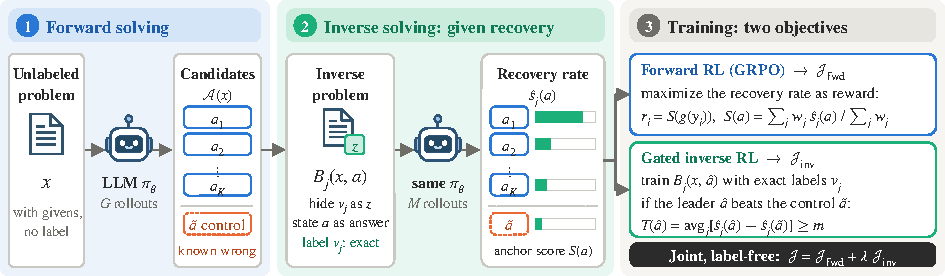
\includegraphics[width=\textwidth]{figures/fig2_method.pdf}
  \caption{One \method step on the problem of Figure~\ref{fig:teaser}. \ding{172}~The distinct answers of $G$ forward rollouts form the candidate set; a perturbed answer serves as a control that is wrong by construction. \ding{173}~For each candidate and each sampled given, a template builds an inverse problem labeled by the hidden given, and the same policy solves it $M$ times. A given's weight is the range of its recovery rates over the candidates. \ding{174}~The weighted recovery rate is the forward reward. The inverse rollouts of the leading candidate enter the loss with exact rewards only if that candidate beats the control by a margin $m$.}
  \label{fig:method}
\end{figure*}

\subsection{Setting and the Consensus Trap}
\label{sec:trap}

A policy $\pi_\theta$ maps a problem $x$ to a response $y$, from which a parser $g$ extracts an answer $a=g(y)$. With a reference answer $\astar$, RLVR assigns $r(y)=\ind[g(y)=\astar]$. GRPO \citep{shao2024deepseekmath} samples $G$ responses per problem, normalizes rewards within the group, $\hat A_i=(r_i-\mathrm{mean}(r_{1:G}))/(\mathrm{std}(r_{1:G})+\epsilon)$, and maximizes
\begin{equation}
\label{eq:grpo}
\mathcal J(\theta)=\E\Big[\frac1G\sum_{i=1}^G\frac{1}{|y_i|}\sum_t\min\big(\rho_{i,t}\hat A_i,\,\bar\rho_{i,t}\hat A_i\big)\Big],
\end{equation}
where $\rho_{i,t}$ is the token-level importance ratio and $\bar\rho_{i,t}$ its clipped value \citep{schulman2017ppo}. In the label-free setting, $\astar$ is hidden during training. We call a problem \emph{confidently wrong} for $\pi_\theta$ if the most frequent sampled answer is incorrect and holds more than half of the samples.

\paragraph{Two-outcome model.}
Fix a problem. The policy outputs $\astar$ with probability $p$ and one aggregate wrong answer $\aminus$ otherwise, and $C\sim\mathrm{Bin}(G,p)$ counts correct rollouts. Let $\zeta\in\{-1,0,1\}$ be the sign of $r(\astar)-r(\aminus)$ in a group. In the small-step limit of GRPO without clipping or KL, each group moves the logit of $p$ by $\zeta\sqrt{C(G-C)}/G$ (Lemma~\ref{lem:common}, Appendix~\ref{app:proofs}), so
\begin{equation}
\label{eq:dyn}
\dot p=\eta\,p(1-p)\,\E\big[\zeta\,\sqrt{C(G-C)}\,/\,G\big].
\end{equation}
Ground-truth rewards give $\zeta=1$ whenever $0<C<G$; agreement-based rewards set $\zeta$ by votes.

\begin{proposition}[Consensus trap]
\label{prop:trap}
If $\zeta$ is decided by the votes of policies whose probabilities of the correct answer all tend to zero with $p$, then $\E[\zeta\sqrt{C(G-C)}]/\E[\sqrt{C(G-C)}]\to-1$, and the all-wrong state is asymptotically stable.
\end{proposition}

Own votes, votes on paraphrases, votes of a peer and a verifier fit to votes all satisfy the hypothesis at the joint all-wrong state, because every vote there favors $\aminus$. Diversity changes how fast correct votes appear as $p$ grows, which moves the basin boundary (Figure~\ref{fig:teaser}b). Escaping the basin needs a signal whose ranking does not depend on what the models believe.

\subsection{Inverse Problems from the Givens}
\label{sec:inverse}

A rule-based parser extracts the given quantities $V(x)=\{v_1,\dots,v_n\}$: numeric literals in the statement outside exponents, indices and the question sentence. A given is eligible if replacing it with a variable leaves another numeric given and a question that names a single quantity (Appendix~\ref{app:givens}). For a candidate answer $a$ and an eligible given $v_j$, the inverse problem $B_j(x,a)$ makes three edits: $v_j$ becomes an unknown $z$, the question becomes a statement that its answer equals $a$, and a new question asks for $z$. Three templates cover quantity, expression and counting questions. The label of $B_j(x,a)$ is $v_j$, exact by construction whether or not $a$ is correct. On DAPO-Math-17k, 83\% of problems have an eligible given and the median problem has three eligible givens; on 200 hand-checked problems, 91\% of parsed eligible givens are correct and 88\% of inverse problems are well posed.

When $a=\astar$, the inverse problem is consistent with $x$ and $v_j$ solves it. When $a$ is wrong, $B_j(x,a)$ is usually still well posed but has another solution ($z\approx3.86$ in Figure~\ref{fig:teaser}a), so a solver that uses the stated answer misses $v_j$. Let $\alpha$ and $\beta$ be the probabilities that one inverse rollout returns $v_j$ under $\astar$ and under the most frequent wrong answer; we call $\Delta=\alpha-\beta$ the \emph{anchor gap}. In the pilot, $\alpha=0.58$, $\beta=0.21$, and a random perturbation of the answer gives $0.12$.

\subsection{Anchor-Scored Forward Reward}
\label{sec:reward}

Let $\cA(x)$ be the $\Kmax$ most frequent distinct parsed answers among the $G$ forward rollouts. With $\Kmax=4$ and $G=8$, $\cA(x)$ contains every parsed answer in 96\% of groups, so a correct minority answer is almost always scored. A control answer $\atilde$ perturbs the most frequent answer (scaling by a factor in $[0.5,1.5]$, or an integer offset in $[-5,5]\setminus\{0\}$) and is resampled until $\atilde\notin\cA(x)$; let $\Aplus(x)=\cA(x)\cup\{\atilde\}$. For $J$ sampled eligible givens and every $a\in\Aplus(x)$, the policy draws $M$ inverse rollouts on $B_j(x,a)$, and $\shat_j(a)$ is the fraction that return $v_j$. The anchor score of a candidate is
\begin{equation}
\label{eq:score}
S(a)=\frac{\sum_j w_j\,\shat_j(a)}{\sum_j w_j},\quad w_j=\max_{\Aplus}\shat_j-\min_{\Aplus}\shat_j ,
\end{equation}
where the maximum and minimum of $\shat_j(a')$ run over $a'\in\Aplus(x)$.
Forward rollout $i$ receives $r_i=S(g(y_i))$ if $g(y_i)\in\cA(x)$ and $r_i=0$ otherwise, including unparsable outputs. A group with $\sum_j w_j<\tau$ is dropped from the batch; with $J=2$, $M=4$ and $\tau=0.5$, this removes groups in which the candidates differ by fewer than two recovered rollouts in total.

\paragraph{Why range weights.}
A problem may state a quantity twice or make it guessable, so some givens are recovered regardless of the answer. Group normalization already removes the bias such a given would cause, because any candidate-independent term in $S$ cancels and an answer-free given adds zero-mean noise to the differences between candidates (Proposition~\ref{prop:noise}). A contrast against the mean recovery over candidates, as in a pointwise-mutual-information score, therefore changes nothing. The remaining cost is variance, which the group standard deviation rescales to full size. The range weight is zero for givens that every inverse rollout recovers and for givens that none recovers, the two common answer-free cases, and $\tau$ drops groups in which no given separates the candidates.

\subsection{Consistency-Gated Inverse Training}
\label{sec:gate}

Inverse rollouts come with exact rewards $\ind[g(\tilde y_k)=v_j]$, so the inverse problems are ordinary RLVR data. Training on all of them would erase the signal. An inverse problem built from a wrong candidate has a solution other than $v_j$, and a rollout that returns $v_j$ there has ignored the stated answer; rewarding it teaches the solver to ignore answers and raises $\beta$ toward $\alpha$. We train only the inverse problems of the leading candidate $\ahat=\arg\max_{a\in\cA(x)}S(a)$, and only when it passes a consistency gate against the control:
\begin{equation}
\label{eq:gate}
T(\ahat)=\frac1J\sum_j\big[\shat_j(\ahat)-\shat_j(\atilde)\big]\ \ge\ m .
\end{equation}
Since the control is wrong by construction, $T$ measures how much stating $\ahat$ helps the solver relative to stating a wrong answer. With $J=2$, $M=4$, $m=0.5$ and the pilot rates, a correct leader passes with probability $0.56$ and a wrong one with probability $0.03$ (Appendix~\ref{app:gate}). The gate also covers groups in which all $G$ rollouts agree. Their forward advantages vanish, as in any GRPO method, and the gate decides whether the single answer is trusted enough to train its inverse problems.

The objective is $\mathcal J_{\text{GivenRL}}=\mathcal J_{\text{fwd}}+\lambda\,\mathcal J_{\text{inv}}$ with $\lambda=0.5$, where $\mathcal J_{\text{fwd}}$ is Eq.~\eqref{eq:grpo} on the kept forward groups with rewards $r_i$, and $\mathcal J_{\text{inv}}$ is Eq.~\eqref{eq:grpo} on the gated inverse groups $B_j(x,\ahat)$ of size $M$ with rewards $\ind[g(\tilde y_k)=v_j]$. With $|\Aplus|=3.4$ on average, scoring adds 27 inverse rollouts per problem at about 40\% of the forward length, and the 8 rollouts of $\ahat$ enter the gradient when the gate passes (Algorithm~\ref{alg:givenrl}).

\subsection{Analysis}
\label{sec:analysis}

In the two-outcome model, each scored given is recovered with probability $\alpha$ under $\astar$ and $\beta$ under $\aminus$, independently across rollouts. Proofs are in Appendix~\ref{app:proofs}.

\begin{theorem}[Unique stable state]
\label{thm:stable}
Let $\psi=P(S(\astar)>S(\aminus))-P(S(\astar)<S(\aminus))$, with dropped groups counted as ties. Under \method's forward reward,
\begin{equation*}
\dot p=\eta\,p(1-p)\,\psi\,\E_{C\sim\mathrm{Bin}(G,p)}\big[\sqrt{C(G-C)}/G\big].
\end{equation*}
If $\psi>0$, the state $p=0$ is unstable and $p(t)\to1$ from every $p(0)\in(0,1)$. If $\alpha>\beta$, then $\psi>0$ for uniform weights and for $J=1$.
\end{theorem}

The update is the ground-truth update scaled by $\psi$ (Figure~\ref{fig:teaser}b), and its sign no longer depends on $p$. For the range weights with $J=2$ and $M=4$, exact enumeration gives $\psi>0.29$ in every cell with $\alpha>\beta$ of a grid with spacing 0.1 over $(\alpha,\beta)$ and three control rates, and $\psi=0.87$ at the pilot rates. Two conditions bound the result. Escape from small $p$ is slow, since $\E[\sqrt{C(G-C)}/G]\approx p\sqrt{G-1}$ gives $\dot p\approx\eta\psi\sqrt{G-1}\,p^2$, so a problem moves only once the correct answer appears among the samples. And the model holds $\alpha$ and $\beta$ fixed while \method trains the inverse solver; Section~\ref{sec:where} measures how both move.

\begin{proposition}[Answer-free givens]
\label{prop:noise}
(i)~Adding to $S(a)$ any quantity that does not depend on $a$ leaves every forward advantage unchanged. (ii)~If $v_j$ is recovered with the same probability $s$ under every candidate, its contribution to $S(a)-S(a')$ has mean zero, and $w_j=0$ almost surely when $s\in\{0,1\}$.
\end{proposition}

\begin{proposition}[Sign error]
\label{prop:sign}
With uniform weights and $J$ givens whose gaps are at least $\Delta$, $P\big(S(\astar)\le S(\aminus)\big)\le\exp(-JM\Delta^2/2)$.
\end{proposition}

At $JM=8$ and the pilot gap $\Delta=0.37$, the bound is $0.58$ and the exact error is $0.09$ (Figure~\ref{fig:analysis}b). The bound gives the rate; the exact value sets the budget.

%=====================================================================
\section{Experiments}
%=====================================================================

\begin{table*}[t]
  \centering
  \footnotesize
  \setlength{\tabcolsep}{4.2pt}
  \begin{tabular}{@{}l cccccccc c cc@{}}
    \toprule
    & \multicolumn{9}{c}{Qwen3.5-4B-Base} & \multicolumn{2}{c}{Avg.} \\
    \cmidrule(lr){2-10}\cmidrule(l){11-12}
    Method & \makecell{AIME\\2024} & \makecell{AIME\\2025} & \makecell{AIME\\2026} & \makecell{HMMT\\2026} & \makecell{AMC\\2023} & \makecell{MATH\\500} & \makecell{Olymp.\\Bench} & \makecell{Minerva\\Math} & Avg. & \makecell{Olmo-3\\7B} & \makecell{Qwen3.5\\9B} \\
    \midrule
    \inputtable{tables/main.tex}
    \bottomrule
  \end{tabular}
  \caption{Math accuracy (\%) after training on DAPO-Math-17k without labels, mean of three seeds. Bold marks the best label-free result per column; gray rows use ground-truth or random rewards and are not ranked. The last two columns give the average on Olmo-3-7B and Qwen3.5-9B-Base; per-benchmark results are in Table~\ref{tab:main_app}. Projected values.}
  \label{tab:main}
\end{table*}

\subsection{Experimental Setup}

\subsubsection{Benchmarks and Baselines}

\paragraph{Data and backbones.}
All methods train on DAPO-Math-17k \citep{yu2025dapo} with every reference answer removed; we use the answers only for evaluation and for the post-hoc diagnostics of Section~\ref{sec:where}. We train Qwen3.5-4B-Base, Qwen3.5-9B-Base \citep{qwen2026qwen35} and Olmo-3-7B \citep{olmo2025olmo3}. Olmo~3 has a public pretraining corpus, which matters because random rewards improve Qwen models on math through memorized content \citep{shao2026spurious} and the Qwen3.5 training data are undisclosed.

\paragraph{Benchmarks and metrics.}
Math: AIME 2024, AIME 2025, AIME 2026, HMMT February 2026, AMC 2023, MATH-500 \citep{hendrycks2021math,lightman2024verify}, OlympiadBench \citep{he2024olympiadbench} and Minerva Math \citep{lewkowycz2022minerva}. Both 2026 contests took place after the release of Olmo~3 and its corpus \citep{balunovic2025matharena}, so they are contamination-free for Olmo-3-7B. Out of domain: GPQA-Diamond \citep{rein2024gpqa}, MMLU-Pro \citep{wang2024mmlupro}, LiveCodeBench v6 \citep{jain2025livecodebench} and both splits of CRUXEval \citep{gu2024cruxeval}, whose input-prediction split asks for a function's input given its output. We report avg@16 on AIME and HMMT, avg@8 on AMC, avg@4 on the other math sets and pass@1 elsewhere (temperature 0.6, top-$p$ 0.95), averaged over three training seeds. The seed standard deviation of the eight-benchmark average is at most 0.31 points for every method (Table~\ref{tab:seeds}).

\paragraph{Baselines.}
From each row of Table~\ref{tab:taxonomy} we take the most recent published method with public code: RENT \citep{prabhudesai2025rent} and Intuitor \citep{zhao2026intuitor}; TTRL \citep{zuo2025ttrl}, EVOL-RL \citep{zhou2025evolrl}, RESTRAIN \citep{yu2026restrain} and OM-GRPO \citep{ye2026omgrpo}; Co-rewarding \citep{zhang2026corewarding} and Self-Harmony \citep{wang2026selfharmony}; and CoVerRL \citep{pan2026coverrl}. Co-RL \citep{yang2026corl} and JURY-RL \citep{chen2026juryrl} need a second policy or a Lean pipeline, so we compare with them at matched compute. GRPO with ground-truth rewards and GRPO with a random reward \citep{shao2026spurious} bracket the table.

\subsubsection{Implementation Details}

All methods use verl \citep{sheng2025hybridflow} with 128 problems per step, $G=8$, learning rate $10^{-6}$, no KL term, clip range 0.2/0.28, 4,096 response tokens and 2 epochs on 16 H100 GPUs per run, and keep the method-specific hyperparameters of their papers. \method uses $\Kmax=4$, $J=2$, $M=4$, $\lambda=0.5$, $\tau=0.5$ and $m=0.5$ throughout, with inverse responses capped at 2,048 tokens (Appendix~\ref{app:impl}).

\subsection{Main Results}
\label{sec:main}



\paragraph{\method is the strongest label-free method on every backbone.}
Its average exceeds the best baseline by 1.6 points on Qwen3.5-4B (OM-GRPO), 1.4 on Olmo-3-7B (CoVerRL) and 2.0 on Qwen3.5-9B (OM-GRPO), and trails ground-truth GRPO by 1.0, 0.8 and 0.9 points (Table~\ref{tab:main}). The lead is largest on the four competition sets. Averaged over AIME 2024 to HMMT 2026, \method reaches 18.2, 9.8 and 23.4 against 16.1, 8.4 and 21.2 for CoVerRL, the strongest baseline there, closing 73\%, 75\% and 65\% of the distance to ground-truth GRPO. Among the baselines, confidence rewards trail vote rewards, and CoVerRL and OM-GRPO lead.

\paragraph{The gain does not come from the backbone.}
The random reward lifts the Qwen3.5 models by 1.8 and 1.7 points and Olmo-3-7B by 0.2, in line with \citet{shao2026spurious}, while \method's gain over the random reward is similar on all three (10.0, 9.6 and 10.7). On Olmo-3-7B, \method raises the contamination-free AIME 2026 from 3.5 to 9.3 and HMMT February 2026 from 1.6 to 4.2, within 0.3 and 0.2 points of ground-truth GRPO (Table~\ref{tab:main_app}).

\begin{table}[t]
  \centering
  \footnotesize
  \setlength{\tabcolsep}{1.9pt}
  \begin{tabular}{@{}l ccccc cc@{}}
    \toprule
    & \multicolumn{5}{c}{Out of domain, pass@1} & \multicolumn{2}{c}{pass@64} \\
    \cmidrule(lr){2-6}\cmidrule(l){7-8}
    Method & GPQA & MMLU & LCB & CX-I & CX-O & A26 & H26 \\
    \midrule
    \inputtable{tables/ood.tex}
    \bottomrule
  \end{tabular}
  \caption{Out-of-domain accuracy and pass@64 (\%) on Qwen3.5-4B-Base after training on math only. MMLU: MMLU-Pro; LCB: LiveCodeBench v6; CX-I/O: CRUXEval input/output prediction; A26/H26: AIME 2026 (30 problems) and HMMT February 2026 (33 problems). Projected values.}
  \label{tab:ood}
\end{table}

\paragraph{Inverse training transfers.}
Trained on math only, \method improves all five out-of-domain suites (Table~\ref{tab:ood}). Its largest gain is on CRUXEval input prediction (+8.5), where it exceeds ground-truth GRPO by 2.2 points, while output prediction, the forward version of the same task, gains 4.9, close to the baselines. Without the inverse term, the input-prediction gain falls to 4.1 and the other suites barely move, which ties the transfer to inverse training.

\paragraph{Coverage at large $k$.}
RLVR often lowers pass@$k$ at large $k$ \citep{yue2025does}. At $k=64$ on the 2026 sets, TTRL solves fewer problems than the base model (9 vs.\ 10 on AIME, 5 vs.\ 6 on HMMT), while \method solves 13 and 9, as many as ground-truth GRPO. Its reward does not favor the most frequent answer. In test-time training on AIME 2026, \method raises avg@16 from 8.1 to 15.8, and in six-epoch runs its MATH-500 accuracy keeps rising while TTRL's falls from 77.8 to 71.2 (Appendix~\ref{app:more}).

\subsection{Ablation Study}
\label{sec:ablation}

\begin{table}[t]
  \centering
  \small
  \setlength{\tabcolsep}{3pt}
  \begin{tabular}{@{}l l c c@{}}
    \toprule
    Variant & Avg. & CW fixed & $\Delta_{\text{end}}$ \\
    \midrule
    \inputtable{tables/ablation.tex}
    \bottomrule
  \end{tabular}
  \caption{One-component ablations on Qwen3.5-4B-Base: math average (change from full), share of confidently wrong problems fixed (\%, Section~\ref{sec:where}), and final anchor gap. Projected values.}
  \label{tab:ablation}
\end{table}

\paragraph{Inverse training needs the gate.}
Table~\ref{tab:ablation} changes one component at a time. Removing the inverse term costs 1.5 points and leaves the anchor gap at its initial 0.37, as does a frozen inverse solver. Training the inverse problems of all candidates is worse than not training them (35.0, $\Delta=0.15$), because the solver learns to recover givens without reading the stated answer. A margin over the runner-up instead of the control gate cannot reject a wrong answer that every rollout agrees on, and the wrong leaders it admits raise $\beta$ from 0.21 to 0.31.

\paragraph{The reward needs every candidate scored.}
Scoring only the two most frequent answers costs 0.8 points and 7 points of fix rate, since a correct answer in third place then receives the minimum reward. Falling back to majority votes on the groups dropped by $\tau$ reintroduces the trap there and lowers the fix rate from 36\% to 30\%. Uniform weights cost 0.3 points and removing the $\tau$ filter 0.6. Inverse problems rewritten by Qwen3.5-27B change the average by 0.1, so templates suffice.

\paragraph{Cost and composition.}
A \method step takes 1.8$\times$ the wall-clock time of a TTRL step. With equal or larger GPU budgets, TTRL and OM-GRPO at $G=16$ reach 33.4 and 36.6, Co-RL with an Olmo-3-7B peer reaches 36.4 at 1.5$\times$ our GPU-hours, and JURY-RL reaches 37.1 at 2.4$\times$ (Table~\ref{tab:matched}). Accuracy tracks $JM$ and saturates near $JM=8$ (Table~\ref{tab:budget}). \method changes the reward, so it composes with methods that change the update: EVOL-RL's novelty bonus gives 38.2 and OM-GRPO's answer masking gives 38.3.

\subsection{Where the Gains Come From}
\label{sec:where}

We sample 16 answers per training problem from Qwen3.5-4B-Base: 14\% of problems are confidently wrong, 61\% confidently right and 25\% uncertain. A problem is fixed if the trained model's most frequent answer is correct, and broken if a confidently right problem ends with a wrong one. Reference answers are consulted only after training.

\begin{table}[t]
  \centering
  \small
  \setlength{\tabcolsep}{2.5pt}
  \begin{tabular}{@{}l ccc ccc@{}}
    \toprule
    & \multicolumn{3}{c}{Fixed / broken (\%)} & \multicolumn{3}{c}{Ranking accuracy} \\
    \cmidrule(lr){2-4}\cmidrule(l){5-7}
    Method & CW & Unc. & CR$\downarrow$ & Step 0 & Final & CW \\
    \midrule
    \inputtable{tables/diag.tex}
    \bottomrule
  \end{tabular}
  \caption{Left: confidently wrong (CW) and uncertain (Unc.) problems fixed, and confidently right (CR) problems broken. Right: fraction of mixed groups in which the reward ranks the correct answer above every incorrect one; ties and dropped groups count one half. TTRL's CW value is zero by definition. Projected values.}
  \label{tab:diag}
\end{table}

\paragraph{Confidently wrong problems.}
The fix rate on confidently wrong problems rises slowly across baselines, from 9\% for TTRL to 22\% for CoVerRL, and jumps to 36\% for \method, against 47\% for ground-truth training (Table~\ref{tab:diag}). Splitting by the initial anchor gap locates the rest of the distance. On the 58\% of these problems with $\Delta>0.1$, \method fixes 50\% and ground-truth GRPO 51\%; on the others, 17\% against 41\%. \method also breaks fewer confidently right problems than any other label-free method.

\paragraph{Ranking accuracy.}
\method ranks the correct answer first in 80\% of mixed groups at initialization, 88\% at the end, and 71\% of confidently wrong groups, where CoVerRL's verifier reaches 21\% because its labels come from the same wrong votes. The two-outcome model at the average pilot gap predicts 94\%; gaps vary across problems, and 29\% of eligible problems start with $\Delta\le0.1$.

\begin{figure}[t]
  \centering
  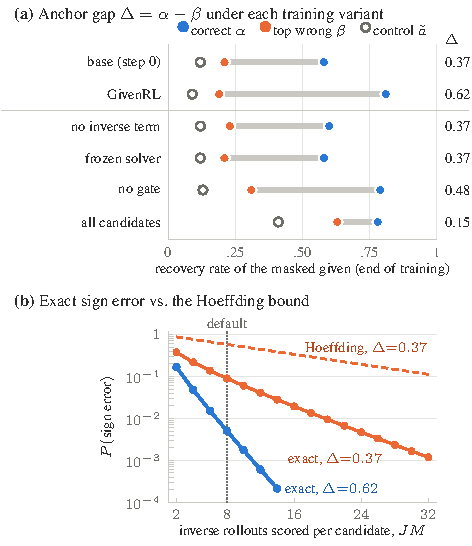
\includegraphics[width=\columnwidth]{figures/fig3_analysis.pdf}
  \caption{\textbf{(a)}~Recovery rates on 512 held-out training problems after training (top row: before training), with the reference answer, the base model's most frequent wrong answer, or a perturbed control written in (projected values). \textbf{(b)}~Probability that the correct answer scores no higher than the wrong one (ties count as errors), computed exactly for uniform weights, against the bound of Proposition~\ref{prop:sign}.}
  \label{fig:analysis}
\end{figure}

\paragraph{Gated inverse training widens the gap.}
On 512 held-out training problems, $\alpha$ rises from 0.58 to 0.81 while $\beta$ stays near 0.2, so $\Delta$ grows from 0.37 to 0.62 (Figure~\ref{fig:analysis}a) and the share of eligible problems with $\Delta>0.1$ grows from 71\% to 84\%. Of the inverse groups that pass the gate, 95\% come from a correct leader. Training all candidates instead lifts $\beta$ to 0.63 and the control to 0.41. A wider gap makes the reward more reliable at a fixed budget: at $JM=8$, the exact sign error falls from 0.09 to 0.005 (Figure~\ref{fig:analysis}b).

%=====================================================================
\section{Conclusion}
%=====================================================================

Agreement-based rewards keep a wrong answer stable however many views they pool, because every view is a belief of the models being trained. A problem's own givens supply a signal from outside those beliefs. They are known exactly, and the correct answer recovers them more often than a wrong one. \method uses this gap to reward forward answers and, under a consistency gate, to train inverse solving with exact labels in the same policy. Other instances of RLVG change how givens are found and checked while keeping the reward of Section~\ref{sec:reward}: symbolic conditions checked by a computer algebra system, hidden test inputs in code, and physical quantities checked for value and unit.

\section*{Limitations}

\method needs problems whose givens can be masked and recovered. On DAPO-Math-17k, 17\% of problems have no eligible given and another 24\% start with an anchor gap below 0.1; \method gets little signal from them, and the share is higher for proofs and open-ended questions. The parser handles numeric givens only. The theory reduces each problem to two outcomes and holds $\alpha$ and $\beta$ fixed; the claim that gated training widens the gap rests on measurements. Escaping a confidently wrong answer requires the correct answer to appear among the samples, which is rare for problems far beyond the model. All training data are math, and a training step costs 1.8$\times$ a TTRL step.

\bibliography{refs}

\appendix

\begin{table*}[t]
  \centering
  \small
  \setlength{\tabcolsep}{5pt}
  \begin{tabular}{@{}l cccccccc c@{}}
    \toprule
    Method & AIME24 & AIME25 & AIME26 & HMMT26 & AMC23 & MATH500 & Olymp. & Minerva & Avg. \\
    \inputtable{tables/main_appendix.tex}
    \bottomrule
  \end{tabular}
  \caption{Per-benchmark math accuracy (\%) on Olmo-3-7B and Qwen3.5-9B-Base, mean of three seeds. Bold marks the best label-free result per column. Projected values.}
  \label{tab:main_app}
\end{table*}

%=====================================================================
\section{Proofs}
\label{app:proofs}
%=====================================================================

\begin{lemma}[Common step]
\label{lem:common}
In the two-outcome model with logit $\ell=\log\frac{p}{1-p}$, one GRPO group with $C$ correct rollouts and reward sign $\zeta$ changes $\ell$ by $\eta\,\zeta\sqrt{C(G-C)}/G$ in the small-step limit without clipping, KL or length normalization; the change is zero if $C\in\{0,G\}$.
\end{lemma}
\begin{proof}
If $\zeta=1$, the normalized advantages are $\sqrt{(G-C)/C}$ for correct and $-\sqrt{C/(G-C)}$ for wrong rollouts; $\zeta=-1$ flips both and $\zeta=0$ zeroes both. Since $\partial_\ell\log\pi(\astar)=1-p$ and $\partial_\ell\log\pi(\aminus)=-p$, the averaged gradient is $\frac{\zeta}{G}\big[C\sqrt{\tfrac{G-C}{C}}(1-p)+(G-C)\sqrt{\tfrac{C}{G-C}}\,p\big]=\zeta\sqrt{C(G-C)}/G$. Multiplying by $\dot\ell$ gives $\dot p=p(1-p)\dot\ell$, which is Eq.~\eqref{eq:dyn}.
\end{proof}

\paragraph{Proposition~\ref{prop:trap}.}
Write $h(C)=\sqrt{C(G-C)}$. Since $h(C)=0$ unless $0<C<G$, it suffices that $P(\zeta=-1\mid 0<C<G)\to1$ as $p\to0$. For own votes, $\zeta=\mathrm{sign}(C-G/2)$, and conditional on $0<C<G$ we have $C=1$ with probability tending to one. For votes of other policies (paraphrases, peers) or of a verifier fit to votes, every vote favors $\aminus$ with probability tending to one at the joint all-wrong state. Hence $\E[\zeta h(C)]/\E[h(C)]\to-1$, and $\dot p<0$ in a neighborhood of $p=0$ for each policy, whose dynamics all take the form of Eq.~\eqref{eq:dyn}. The all-wrong state is therefore asymptotically stable.

\paragraph{Theorem~\ref{thm:stable}.}
In the two-outcome model with $0<C<G$, both answers are in $\cA(x)$ and share the control $\atilde$. The sign $\zeta=\mathrm{sign}(S(\astar)-S(\aminus))$ is a function of the inverse rollouts only, which are independent of $C$, so $\E[\zeta h(C)]=\psi\,\E[h(C)]$ and Eq.~\eqref{eq:dyn} gives the stated dynamics. If $\psi>0$, then $\dot p>0$ on $(0,1)$; $p(t)$ increases and is bounded, and its limit is a zero of $\dot p$ in $(p(0),1]$, which is only $1$. For uniform weights, $\zeta=\mathrm{sign}(X-Y)$ with $X\sim\mathrm{Bin}(JM,\alpha)$, $Y\sim\mathrm{Bin}(JM,\beta)$ independent. Pairing each outcome $(x,y)$ with $x>y$ with its swap $(y,x)$, the likelihood ratio is $\big[\alpha(1-\beta)/(\beta(1-\alpha))\big]^{x-y}>1$ when $\alpha>\beta$, so $P(X>Y)>P(X<Y)$. For $J=1$ with any weight, $w_1$ is symmetric in the two candidates and cancels in the sign, so the same argument applies. For range weights with $J\ge2$ the exponent of the likelihood ratio is the unweighted count difference, which can disagree in sign with the weighted one; we therefore evaluate $\psi$ by exact enumeration over all $(M+1)^{3J}$ outcomes (Section~\ref{sec:analysis}).

\paragraph{Proposition~\ref{prop:noise}.}
(i)~GRPO advantages are invariant to adding a constant to every reward in a group. (ii)~If $\shat_j(a)$ and $\shat_j(a')$ are i.i.d., exchanging them leaves $w_j$ and $\sum_k w_k$ unchanged and negates $w_j(\shat_j(a)-\shat_j(a'))/\sum_k w_k$, so its mean is zero. If $s\in\{0,1\}$, every $\shat_j$ equals $s$ and the range is zero.

\paragraph{Proposition~\ref{prop:sign}.}
$(X-Y)/(JM)$ is a mean of $JM$ independent terms in $[-1,1]$ with mean at least $\Delta$. Hoeffding's inequality gives $P(X-Y\le0)\le\exp\!\big(-2JM\Delta^2/4\big)=\exp(-JM\Delta^2/2)$.

\subsection{Gate Pass Probabilities}
\label{app:gate}
With homogeneous givens, $\sum_j\shat_j(\ahat)\cdot M\sim\mathrm{Bin}(JM,q)$ and $\sum_j\shat_j(\atilde)\cdot M\sim\mathrm{Bin}(JM,\gamma)$, and Eq.~\eqref{eq:gate} with $m=0.5$ asks the first count to exceed the second by at least $mJM=4$. At the pilot rates ($\gamma=0.12$), the pass probability is $0.56$ for a correct leader ($q=\alpha=0.58$) and $0.03$ for a wrong one ($q=\beta=0.21$); at the end-of-training rates ($0.81$, $0.19$, $0.09$) it is $0.94$ and $0.03$.

%=====================================================================
\section{Givens, Eligibility and Templates}
\label{app:givens}
%=====================================================================

The parser marks numeric literals in the problem statement as givens. It skips exponents, subscripts and indices, numbers in the final question sentence, numbers inside figure environments, and numbers that are part of a named constant. A given is eligible if, after replacement by $z$, the statement still contains another numeric given and the question names a single quantity. Each inverse problem uses one of three templates, chosen by the question sentence:
\begin{enumerate}[leftmargin=*,itemsep=1pt,topsep=2pt]
  \item \emph{Quantity} (``How much \dots'', ``What is \dots''): replace $v_j$ with $z$, turn the question into ``The answer to this question is $a$.'', and append ``What is the value of $z$?''
  \item \emph{Expression} (``Find \dots'', ``Compute \dots''): replace $v_j$ with $z$ and append ``It is known that the requested quantity equals $a$. Find $z$.''
  \item \emph{Count} (``How many \dots''): as template 1, with ``There are exactly $a$ such \dots'' as the answer sentence.
\end{enumerate}
If an inverse problem admits several values of $z$, a rollout counts as correct only when it returns $v_j$, which lowers $\alpha$ for that given; the weights down-rank such givens. Template outputs for three illustrative problems:

\begin{small}
\begin{itemize}[leftmargin=*,itemsep=2pt,topsep=2pt]
  \item \emph{Quantity.} $x$: ``A train travels 240 km in 3 hours. What is its average speed in km/h?'' With $a=80$ and $v_j=240$: ``A train travels $z$ km in 3 hours. The answer to this question is 80. What is the value of $z$?'' (label 240).
  \item \emph{Expression.} $x$: ``Let $f(t)=2t+5$. Compute $f(7)$.'' With $a=19$ and $v_j=5$: ``Let $f(t)=2t+z$. It is known that the requested quantity equals 19. Find $z$.'' (label 5).
  \item \emph{Count.} $x$: ``How many positive divisors does 36 have?'' The only given sits in the question sentence, so the problem has no eligible given and receives no forward signal.
\end{itemize}
\end{small}

%=====================================================================
\section{Implementation Details}
\label{app:impl}
%=====================================================================

\begin{table}[H]
  \centering
  \small
  \setlength{\tabcolsep}{4pt}
  \begin{tabular}{@{}ll@{}}
    \toprule
    Setting & Value \\
    \midrule
    Framework & verl \\
    Problems per step & 128 \\
    Forward rollouts $G$ & 8 \\
    Learning rate & $10^{-6}$, constant \\
    KL coefficient & 0 \\
    Clip range (low / high) & 0.2 / 0.28 \\
    Max tokens & 4,096 forward, 2,048 inverse \\
    Epochs & 2 (6 in Table~\ref{tab:long}) \\
    Temperature & 1.0 training, 0.6 evaluation \\
    \method: $\Kmax$, $J$, $M$ & 4, 2, 4 \\
    \method: $\lambda$, $\tau$, $m$ & 0.5, 0.5, 0.5 \\
    Control $\atilde$ & scale by $U[0.5,1.5]$; integers: \\
     & offset in $[-5,5]\setminus\{0\}$ \\
    Hardware & 16 H100 GPUs per run \\
    \bottomrule
  \end{tabular}
  \caption{Hyperparameters.}
  \label{tab:hparams}
\end{table}

\begin{algorithm}[H]
\caption{One \method step}
\label{alg:givenrl}
\small
\begin{algorithmic}[1]
\For{each problem $x$ in the batch}
  \State Sample $G$ forward rollouts; parse answers; form $\cA(x)$ and the control $\atilde$
  \State Sample $J$ eligible givens; for each $a\in\Aplus(x)$ build $B_j(x,a)$ and draw $M$ inverse rollouts
  \State Compute $\shat_j(a)$, $w_j$ and $S(a)$ (Eq.~\ref{eq:score})
  \If{$\sum_j w_j\ge\tau$} add the forward group with rewards $S(g(y_i))$ \EndIf
  \If{$T(\ahat)\ge m$ (Eq.~\ref{eq:gate})} add the inverse groups of $\ahat$ with rewards $\ind[g(\tilde y_k)=v_j]$ \EndIf
\EndFor
\State Normalize advantages per group and take one step on $\mathcal J_{\text{fwd}}+\lambda\,\mathcal J_{\text{inv}}$
\end{algorithmic}
\end{algorithm}

%=====================================================================
\section{Additional Results}
\label{app:more}
%=====================================================================

All values in this appendix are projected.



\begin{table}[H]
  \centering
  \small
  \setlength{\tabcolsep}{5pt}
  \begin{tabular}{@{}lccc@{}}
    \toprule
    Method & Qwen-4B & Olmo-7B & Qwen-9B \\
    \midrule
    \inputtable{tables/seeds.tex}
    \bottomrule
  \end{tabular}
  \caption{Standard deviation of the eight-benchmark average over three training seeds (over three evaluation seeds for the base model). Projected values.}
  \label{tab:seeds}
\end{table}

\begin{table}[H]
  \centering
  \small
  \setlength{\tabcolsep}{4pt}
  \begin{tabular}{@{}cccc cc@{}}
    \toprule
    $\Kmax$ & $J$ & $M$ & $JM$ & Avg. & Step time vs.\ TTRL \\
    \midrule
    \inputtable{tables/budget.tex}
    \bottomrule
  \end{tabular}
  \caption{Budget sensitivity on Qwen3.5-4B-Base. The default (shaded) is within 0.3 points of the best setting at 69\% of its step time. Projected values.}
  \label{tab:budget}
\end{table}

\begin{table}[H]
  \centering
  \small
  \setlength{\tabcolsep}{3pt}
  \begin{tabular}{@{}llcc@{}}
    \toprule
    Method & Setting & GPU-h & Avg. \\
    \midrule
    \inputtable{tables/matched.tex}
    \bottomrule
  \end{tabular}
  \caption{Comparison at matched compute on Qwen3.5-4B-Base. GPU-hours are relative to \method; Co-RL counts both policies. Projected values.}
  \label{tab:matched}
\end{table}

\begin{table}[H]
  \centering
  \small
  \begin{tabular}{@{}lcc@{}}
    \toprule
    Method & AIME 2026 & HMMT Feb 2026 \\
    \midrule
    \inputtable{tables/ttt.tex}
    \bottomrule
  \end{tabular}
  \caption{Test-time training on the unlabeled test problems (Qwen3.5-4B-Base), avg@16, mean $\pm$ standard deviation over five seeds. Projected values.}
  \label{tab:ttt}
\end{table}

\begin{table}[H]
  \centering
  \small
  \setlength{\tabcolsep}{3pt}
  \begin{tabular}{@{}lccccc@{}}
    \toprule
    & \multicolumn{3}{c}{MATH-500 at epoch} & Length & Reward \\
    \cmidrule(lr){2-4}
    Method & 2 & 4 & 6 & 2$\to$6 & std ratio \\
    \midrule
    \inputtable{tables/long.tex}
    \bottomrule
  \end{tabular}
  \caption{Six-epoch training on Qwen3.5-4B-Base: MATH-500 accuracy, change in mean response length, and within-group reward standard deviation at epoch 6 relative to its initial value. Projected values.}
  \label{tab:long}
\end{table}

\end{document}
